\chapter{Исследовательская часть}

В данном разделе будут приведены примеры работы программы, и будет проведен сравнительный анализ реализаций алгоритма по затраченному процессорному времени.

\section{Технические характеристики}

Технические характеристики устройства, на котором выполнялось исследование, приведены ниже:

\begin{itemize}
	\item операционная система Manjaro Linux \cite{manjaro};
	\item память 7,6 ГБ;
	\item процессор 8 × Intel® Core™ i5-10210U CPU @ 1.60 ГГц \cite{intel} c 4 физическими ядрами и 8 логическими.
\end{itemize}

\clearpage

\section{Демонстрация работы программы}

На рисунке \ref{img:example} приведен пример работы программы. На этом рисунке пользователь выбирает из меню пункт 1 --- однопоточную реализацию алгоритма, вводит Q и размерность матрицы и получает на выходе набор матриц, в каждой из которых значения элементов <= k, где $k\in [1,Q]$.

\begin{figure}[H]
	\begin{center}
		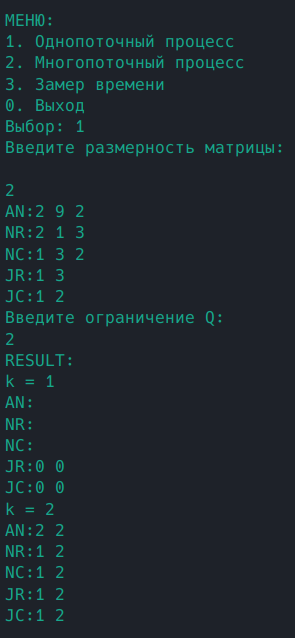
\includegraphics[scale=1]{img/example.png}
	\end{center}
	\captionsetup{justification=centering}
	\caption{Пример работы программы}
	\label{img:example}
\end{figure}

\section{Временные характеристики}

Функция $std::chrono::system\_clock::now(...)$ из библиотеки $chrono$ языка программирования $C++$ возвращает  процессорное время в секундах --- значение типа float.

На рисунке \ref{img:time} приведены результаты замеров времени выполнения однопоточной и многопоточной  реализаций заданного алгоритма.

\begin{figure}[H]
	\begin{center}
		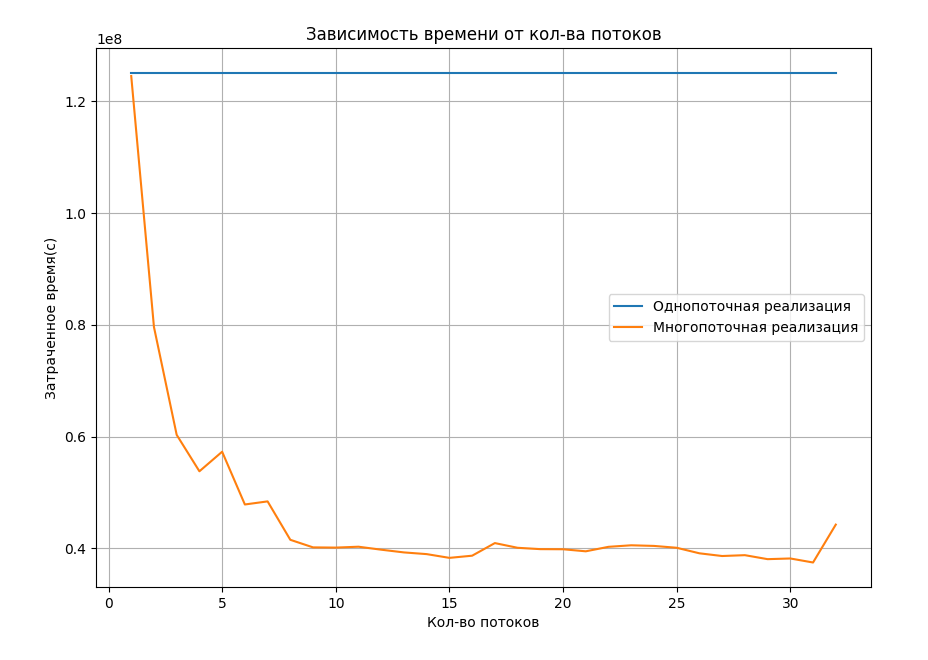
\includegraphics[scale=0.6]{img/time.png}
	\end{center}
	\captionsetup{justification=centering}
	\caption{Сравнение времени выполнения реализаций алгоритмов}
	\label{img:time}
\end{figure}

\section{Вывод}
Приведенные характеристики времени показывают, что многопоточная реализация выигрывает по времени у последовательной реализации, достигается ускорение в 3 раза.